\subsection{PLC}
This section should be a general description of a particular subsystem for the given layer. For most subsystems, an extract of the architectural block diagram with data flows is useful. This should consist of the subsystem being described and those subsystems with which it communicates.

\begin{figure}[h!]
	\centering
 	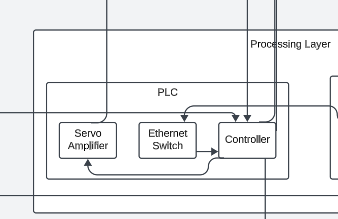
\includegraphics[width=0.60\textwidth]{images/PLC.png}
 \caption{PLC subsystem.}
\end{figure}

\subsubsection{Assumptions}
PLC is like a central processing unit of this product. The input comes from the input layer. Then, the input is processed and sent to the output layer. 

\subsubsection{Responsibilities}
PLC consists of many components. But the three major components are the Servo amplifier, Ethernet switch, and Controller. 
Servo amplifier: The Servo amplifier's job is to move the linear rail into the appropriate position so that the arm can perform its targeted operation (picking box). The amplifier sends a signal from the Controller because it is connected as an additional axis to the controller beside other joints of the robot arm.
Ethernet Switch: The ethernet switch is present inside the controller. Since this robot is being controlled via TCP/IP, it is very important to have a stable wired connection. This switch makes communication possible between the PC and the Controller.
Controller: The controller, as the name sounds, controls the robot arm and rail. The instructions or commands it takes as input from the PC result in the movement of the robot arm accordingly. The controller also generates output to other parts of the product. It sends signals continuously to the indicator, indicating the robot status. Green is working correctly. Orange attention is required. Red stopped working. It instructs the arm when to align all the joints and pick the box using a gripper. 

\subsubsection{Subsystem Interfaces}
\begin {table}[H]
\caption {Subsystem interfaces} 
\begin{center}
    \begin{tabular}{ | p{1cm} | p{3cm} | p{6cm} | p{6cm} |}
    \hline
    ID & Description & Inputs & Outputs \\ \hline
    \#1 & Takes input from controller & \pbox{3cm}{ Controller } & \pbox{6cm}{Movement of Linear Rail}  \\ \hline
    \#2 & Takes input from PC & \pbox{3cm}{PC} & \pbox{4cm}{Send signal to Controller}  \\ \hline
    \#3 & Takes input from different components & \pbox{6cm}{a. Input from PC via ethernet switch \\b. Input from gate sensor \\c. Input from E-Stops } & \pbox{6cm}{a)	Sends the signal to servo amplifier and align joints to perform action.\\b)	If the gate sensor is triggered, arm operation is terminated\\c)	If e-stops are hit, arm operations are terminated
}  \\ \hline
    \end{tabular}
\end{center}
\end{table}

